\documentclass[show notes on second screen=right]{beamer}
\usepackage{listings}
\usepackage{tikz}
\usepackage{hyperref}
\hypersetup{
    colorlinks=true,
    linkcolor=blue,
    urlcolor=blue,
    citecolor=blue
}

\setbeamertemplate{footline}[frame number]

\titlegraphic{
  \begin{center}
    
\includegraphics[width=0.5\textwidth]{./../src/GitLogo.png}
  \end{center}
}
\title{Git Introduction Course}
\author{Romain De Groote}
\date{\today}

\setbeamerfont{title}{size=\Huge,series=\bfseries}

\setbeamertemplate{title page}{
  \begin{centering}
    \vspace*{0.3cm}
    {\usebeamerfont{titlegraphic}\inserttitlegraphic\par}
    \vspace{-0.1cm}
    {\usebeamerfont{title}\inserttitle\par}
    \vspace{0.2cm}
    {\usebeamerfont{author}\insertauthor\par}
    {\usebeamerfont{date}\insertdate\par}
  \end{centering}
}

\begin{document}

\begin{frame}
\titlepage
\note{
  \begin{itemize}
    \item Introducing the course and myself
    \item english course, question en or fr (german not localized yet)
    \item thanking everyone for attending
    \item explaining the structure of the course and what we will cover
    \item encouraging questions
    \item interactive course (lot of practise and installation)
    \item course not exhaustive, but provide solid basis
  \end{itemize}
}
\end{frame}

\section{Why Git?}
\begin{frame}[t]{Why Git?}
  \onslide<+->
  Git offer many benefits for developers and teams, including:
  \onslide<+->
  \begin{itemize}
    \item Share code with others
    \item Track changes
    \item Revert to previous versions
    \item Collaborate effectively
    \item Designed to be fast, efficient, and scalable
    \item Widely used in the software development industry \note{speak about some project (Mistrail AI, python, Linux Kernel, etc.)}
  \end{itemize}
  \onslide<+->
  Why not:
  \begin{itemize}
    \item Use a shared folder?
    \item Use a cloud storage service?
    \item USB stick?
  \end{itemize}
  \note{Share folder:
  \begin{itemize}
    \item No history, no tracking, limited collaboration, always depending on online access
  \end{itemize}
  Cloud storage:
  \begin{itemize}
    \item No history, no tracking, limited collaboration, always depending on online access, security issues
  \end{itemize}
  USB stick:
  \begin{itemize}
    \item No history, no tracking, limited collaboration, security issues, risk of loss/damage, inconvenient to share
  \end{itemize}}
  \onslide<+->
  Real difficulty: organization between the members to know who works on what, and to avoid conflicts when merging changes.\\
\end{frame}

\section{Starting up}
\begin{frame}[t]{Starting up}
  \onslide<+->
  \begin{itemize}
    \item Install Git
    \begin{itemize}
      \item www.git-scm.com/downloads
    \end{itemize}
    \onslide<+->
    \item Setting up Git
    \onslide<+->
    \item Create GitHub/GitLab account
    \begin{itemize}
      \item GitHub: github.com/join
      \item GitLab: gitlab.com/users/sign\_up
    \end{itemize}
    \onslide<+->
    \item (Overleaf)
  \end{itemize}
  \onslide<+->
  Online systems are not protected from all vulnerabilities, so try to always have a local copy of your most important works.\\
  \href{https://www.githubstatus.com/uptime/hhtssxt0f5v2}{GitHub status}\\
  \href{https://status.gitlab.com}{GitLab status}
  \note{Take time to create accounts with Github^|Gitlab, and installing Git on computer}
\end{frame}

\section{Cloning a repository}
\begin{frame}[t]{Cloning a repository}
  Practise exercise:
  \begin{itemize}
    \item Open Git Bash
    \item Use \texttt{cd <path>} to navigate to the folder where you want to clone the repository
    \begin{itemize}
      \item try \texttt{ls} to list the content of the folder and \texttt{cd ..} to go back to the parent folder
    \end{itemize}
    \item Use \texttt{git clone https://github.com/MatsuneMikuroi\\/GitCrashCourse.git <folder\_name>} to clone the repository into a specific folder
  \end{itemize}
\end{frame}

\section{Initializing a repository}
\begin{frame}[t]{Initializing a repository}
  Practise exercise:
  \begin{itemize}
    \item Open Git Bash
    \item Use \texttt{cd <path>} to navigate to the folder where you want to initialize the repository
    \item Use \texttt{git init} to initialize a new Git repository
  \end{itemize}
\end{frame}

\section{Branching}
\begin{frame}[t]{Branching}
  Branches allows you to:
  \begin{itemize}[<+->]
    \item Work on different version of a same file
    \item Create a new copy where you can test/experiment
    \item Merge the changes if you are satisfied
  \end{itemize}
  \onslide<+->
  The main branch (good practice):
  \begin{itemize}
    \item Core of the project
    \item Stable version only
    \item Only merge when you are sure the changes are good
  \end{itemize}
\end{frame}

\section{Working with branches}
\begin{frame}[t]{Working with branches}
  Practise exercise:
  \begin{itemize}
    \item Go the folder where you initialized the repository
    \item Create a .txt file and add some content to it
    \item Use \texttt{git add <file\_name>} to stage the file
    \item Use \texttt{git commit -m "Initial commit"} to commit the changes
    \item Use \texttt{git branch <branch\_name>} to create a new branch
    \item Use \texttt{git checkout <branch\_name>} to switch to the new branch
    \item Make some changes to the .txt file and commit the changes
    \item Use \texttt{git checkout main} to switch back to the main branch
    \item Use \texttt{git merge <branch\_name>} to merge the changes from the new branch to the main branch
    \item Use \texttt{git branch -d <branch\_name>} to delete the new branch
  \end{itemize}
\end{frame}

\begin{frame}[t]{Working with branches (cont.)}
  With all this, you should have a Git history that looks like this:
  \begin{center}
  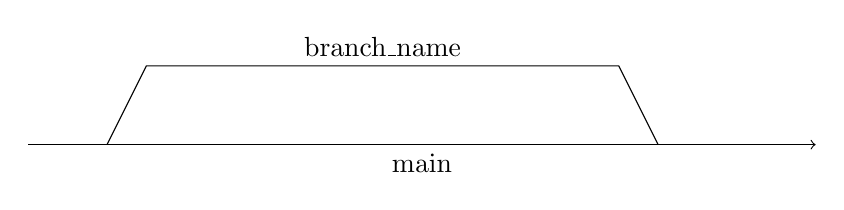
\begin{tikzpicture}
    \draw[->] (0,0) -- (10,0) node [midway, below] {main};
    \draw (1,0) -- (1.5,1) -- (7.5,1) node [midway, above] {branch\_name} -- (8,0);
  \end{tikzpicture}
  \end{center}
  \onslide<+->
  Be cautious, \texttt{git merge} merge the selected branch into the current branch, try to avoid this:
  \onslide<+->
  \begin{figure}
    \centering
    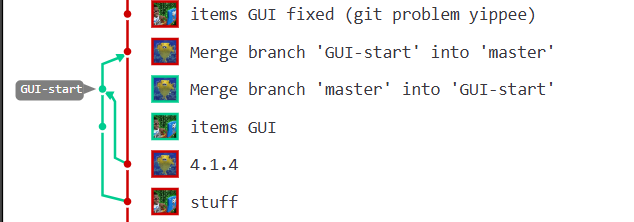
\includegraphics[width=\textwidth]{./../src/panic.png}
  \end{figure}
\end{frame}

\section{Linking local and remote}
\begin{frame}
  \centering
  \Huge Linking local and remote\\
  \LARGE (IDE and Desktop app)
\end{frame}

\subsection{Github Desktop}
\begin{frame}[t]{Github Desktop}
  If you want to work with Github and have a nice GUI:
  \begin{itemize}
    \item Dowload Github Desktop: \url{https://desktop.github.com/}
    \item Link your Github account
    \item Clone the repository you created in the previous exercises
    \item Make some changes to the .txt file and commit the changes
    \item Push the changes to the remote repository
    \item Go to the Github website and check that the changes are there
  \end{itemize}
\end{frame}

\subsection{Git Kraken}
\begin{frame}[t]{Git Kraken}
  If you want to work with GitLab/Github/Gitbucket and have a nice GUI:
  \begin{itemize}
    \item Dowload Git Kraken: \url{https://www.gitkraken.com/}
    \item Link your Github/GitLab/Gitbucket account
    \item Clone the repository you created in the previous exercises
    \item Make some changes to the .txt file and commit the changes
    \item Push the changes to the remote repository
    \item Go to the Github/GitLab/Gitbucket website and check that the changes are there
  \end{itemize}
  \note{Github desktop is only for Github, while Git Kraken support multiple platforms. However Github desktop is free, while Git Kraken is not (but have a free version with limited features)}
\end{frame}

\subsection{IDE}

\begin{frame}[t]{IDE}
  In most IDE, you can link your GitHub/GitLab account and work with Git directly from the IDE.\\
  \begin{itemize}
    \item Visual Studio Code
    \item JetBrains IDEs (PyCharm, IntelliJ, etc.)
    \item Eclipse
  \end{itemize}
  \note{See with students which IDE they are using and show them how to link their GitHub/GitLab account and work with Git from the IDE}
\end{frame}

\subsection{SSH keys and Personal Access Tokens (PAT)}
\begin{frame}[t]{SSH keys and Personal Access Tokens (PAT)}
  \onslide<+->
  When you want to push your changes to a remote repository, you need to authenticate yourself.\\
  \onslide<+->
  \begin{itemize}
    \item SSH keys
    \begin{itemize}
      \item More secure than username/password
      \item Can be used for multiple repositories
      \item Can be used for multiple platforms (Github, GitLab, etc.)
    \end{itemize}
    \onslide<+->
    \item Personal Access Tokens (PAT)
    \begin{itemize}
      \item Used when SSH keys are not supported (e.g., Overleaf)
      \item Can be used for multiple repositories and platforms (Github, GitLab, etc.)
      \item Less secure than SSH keys, but still better than username/password
      \item Can be revoked at any time
      \item Can have specific permissions (e.g., read-only, write-only, etc.)
      \item Can be used for automation (e.g., CI/CD pipelines, scripts, etc.)
      \item Can be used for third-party applications (e.g., Overleaf, etc.)
    \end{itemize}
  \end{itemize}
  \note{Show how to generate SSH keys and Personal Access Tokens (PAT) on Github/GitLab and how to use them to authenticate yourself when pushing changes to a remote repository}
  \note{If using desktop GUI, just login with your account and the authentication will be handled automatically, no need to generate SSH keys or PAT\\
  Show some example by loging to Github/GitLab from git kraken}
\end{frame}

\begin{frame}{}
  \onslide<+->
  \begin{center}
  \huge \color{red} NEVER SHARE YOUR SSH KEYS OR PAT WITH ANYONE
  \end{center}
  \normalsize
  \ 
  \onslide<+->
  \begin{itemize}
    \item Scope your PAT at the strict minimum permissions you need
    \item If risks of compromise, revoke the PAT/SSH key and generate a new one immediately
    \item If you accidentally commit your PAT/SSH key to a Git repository, remove it from the history and revoke it immediately
    \item Add collaborators to your repository with the appropriate permissions
    \item If you really need to add a PAT/SSH key, add it as a secret\note{Show example of how to add a secret in GitHub/GitLab}
  \end{itemize}
  \note{show how to add secret in GitHub/GitLab}
\end{frame}

\section{Conclusion}

\begin{frame}[t]{Conclusion}
  \begin{itemize}
    \item Git is a powerful tool for version control and collaboration
    \item It is widely used in the software development industry
    \item It can be used with different platforms (Github, GitLab, etc.) and tools (IDE, desktop app, etc.)
    \item It is important to understand the basics of Git to work effectively with it
    \item Always keep a local copy of your most important works and be cautious when sharing your SSH keys or PAT
  \end{itemize}
\end{frame}

\begin{frame}[t]{To go further}
  \begin{itemize}
    \item Markdown files and documentation
    \item `.gitignore` files
    \item Seeting up a Git server locally
  \end{itemize}
\end{frame}

\end{document}